\documentclass[12pt,a4paper]{article}
\usepackage{enumerate}
\usepackage{fullpage}
\usepackage{amsmath}
\usepackage{graphicx}
\usepackage{verbatim}
\usepackage{parskip}

% Stuff for dot2tex
\usepackage[x11names, rgb]{xcolor}
\usepackage[utf8]{inputenc}
\usepackage{tikz}
\usetikzlibrary{snakes,arrows,shapes}


\title{Stats 391 Project}
\author{By \\ Henry Baba-Weiss, Bill Cauchois, Coral Peterson, and Michael Sloan}
\date{\today}

\begin{document}

\maketitle
\pagebreak

\section { Background }

Tweets are very short messages posted to the online micro-blogging service Twitter. By convention less than 140 characters in length, tweets may also contain Twitter-specific idioms such as hashtags and @ mentions.  The brevity and concision of Twitter make it a potentially interesting source of information for applying more naive statistical methods and learning techniques.  Many of the Tweets are written to be consumed without additional context, making them ideal targets for more simplistic statistical methods.

\section { Description }

The goal of our project is to apply statistical tools to build a model which predicts the ``sentiment'' of tweets.  This sentiment is dichotomized into just two categories: ``positive'' and ``negative''.  The positive category is used for posts that would otherwise go into a neutral category, if it existed.

We used Naive Bayes as our statistical model. We relied upon a variety of methods for data collection and labeling, to create our training and test corpuses.


\section { Maths }

\subsection { Naive Bayes }

The ``Naive Bayes classifier'' takes the following form:

\begin{align*}
p(C \vert F_1,\dots,F_n) = \frac{1}{Z}  p(C) \prod_{i=1}^n p(F_i \vert C)
\end{align*}

This formula comes from assuming that the conditions, $ F_n $, are independent.  The $ Z $ is a scaling factor, which is irrelevant for the purposes of comparison.  This allows us to extract the compound probability, $ p(F_1,\cdots,F_n) = \prod_{i=1}^n p(F_i) $ from the usual formula for Bayes' theorem:

\begin{align*}
p(C \vert F_1,\dots,F_n) & = \frac{p(C) p(F_1,\dots,F_n\vert C)}{p(F_1,\dots,F_n)}    \\
                         & \approx \frac{p(C) \prod_{i=1}^n p(F_i \vert C)}{p(F_1,\dots,F_n)} \\
                         & \approx \frac{p(C) \prod_{i=1}^n p(F_i \vert C)}{Z}
\end{align*}
(Where $ Z = p(F_1,\cdots,F_n) $ )

In essence, this means that the likelihood of a given outcome is the product of the probabilities contributed by each of the predictors.  $ Z $ can be disregarded, because usually we are interested in comparing two outcomes.  For our usage here, we will assume that $ C_1 $ and $ C_2 $ are disjoint, which is given by our problem statement dichotomizing ``Positive'' and ``Negative'' sentiment.  In order to figure out which is more likely given all of $F_n$, we could calculate:

\begin{align*}
  & \frac{\displaystyle p(C_1 \vert F_1,\dots,F_n) } { P(C_1 \vert F_1,\dots,F_n) + P(C_2 \vert F_1,\dots,F_n) } \\
  & \\
  \approx & \frac{\displaystyle \frac{\displaystyle p(C_1) \prod_{i=1}^n p(F_i \vert C_1)}{\displaystyle Z}}{\frac{\displaystyle p(C_1) \prod_{i=1}^n p(F_i \vert C_1)}{\displaystyle Z} + \frac{\displaystyle p(C_2) \prod_{i=1}^n p(F_i \vert C_2)}{\displaystyle Z}} \\
  & \\
  \approx & \frac{\displaystyle p(C_1) \prod_{i=1}^n p(F_i \vert C_1)}{p(C_1) \prod_{i=1}^n p(F_i \vert C_1) + p(C_2) \prod_{i=1}^n p(F_i \vert C_2)}
\end{align*}

This results in a distribution on a discrete binary variable (the denominator specifies the domain that we're concerned with - we must be inhabiting either $ C_1 $ or $ C_2 $).  The assumption that $ C_1 $ and $ C_2 $ are disjoint allows us to express the overall probability of inhabiting the 

$ p(C_1) $ is referred to as the ``prior'', or the probability of $ C_1 $, regardless of other information.  This is an interesting aspect of the Naive Bayes classifier - achieving better results by ``starting'' with an appropriately biased assumption.

Our actual implementation does not use this form of the equation, as we're more interested in the comparison between $ P(C_1 \vert F_1,\dots,F_n) $, rather than their absolute values.  As such, we can take a log of both sides, while maintaining ordering (of positive values, which probabilities are):

\begin{align*}
p(C_1 \vert F_1,\dots,F_n) & \stackrel{\text{?}}{\leq} p(C_2 \vert F_1,\dots,F_n) \\
log p(C_1 \vert F_1,\dots,F_n) & \stackrel{\text{?}}{\leq} log p(C_2 \vert F_1,\dots,F_n) \\
log p(C_1) \prod_{i=1}^n p(F_i \vert C_1) & \stackrel{\text{?}}{\leq} log p(C_2) \prod_{i=1}^n p(F_i \vert C_2) \\
log p(C_1) + \sum_{i=1}^n log p(F_i \vert C_1) & \stackrel{\text{?}}{\leq} log p(C_2) + \sum_{i=1}^n log p(F_i \vert C_2) \\
\end{align*}

\subsection { Connections to Advanced Topics }

\section{ Implementation }

The implementation of our project can be broadly divided into several different components. Before performing any classification, we first had to collect data and then label that data. We implemented a \textbf{scraper} in Python to aggregate raw tweets from Twitter's feed of recent tweets. Next, we used several different methods to label the tweets as positive or negative in order to create a training set for our classifier. These methods included \textbf{Mechanical Turk}, a web-based service that lets you pay others to perform classification; \textbf{manual console categorization}, wherein we manually classified tweets using a console program; and \textbf{manual web-based categorization}, wherein we manually classified tweets using a web application. Now that we had labeled data, the next challenge was \textbf{lexing} that data to create a bag of words representation for each tweet. Finally, we built our \textbf{Bayesian categorizer}. We also built a \textbf{web frontend}.

\subsection { Scraper }

The first component we built was a scraper to grab random tweets from Twitter. To do so, we used the \texttt{twitter.Api().GetPublicTimeline()} method on the Twitter Python API, which in turn uses HTTP REST to grab the most recent tweets from the public, global timeline. One problem we ran into was that not all of these tweets were in English. In order to discard tweets that weren't in English, we relied upon a Java library called TextCat that performs text categorization into different languages. So we created a small program that read in a tweet, and outputted the language in which that tweet was written. Then, we could call into this program from Python and use it to discard any tweet for which the output from TextCat was \emph{not} ``english''. The output from our scraper was stored in comma-separated values format. Here is an example listing (including the header):

\begin{verbatim}
name,text
Marcus Graham ,Go somewhere then RT @NurseJessica_88: Im seriously needing to get out the house
Brett taborelli,Here it goes.
Jessica Stein,Thank god I'll be waking up in sea isle instead of havertown tomorrow
\end{verbatim}

\subsection { Mechanical Turk }

Our first approach to solving the problem of labeling our tweets relied upon a service called Mechanical Turk. Mechanical Turk bills itself as ``an online crowdsourcing marketplace''. Crowdsourcing is a recently coined term that refers to outsourcing tasks to a distributed group of people, usually via the internet. Basically, MTurk enables users known as Requesters to post tasks known as HITs (human intelligence tasks) for a distributed force of Workers to perform for a small fee. There are several different types of HITs, but the type we were interested in was the classification HIT, wherein a Worker assigns one of $n$ categories to a piece of data. MTurk turned out to be relatively easy to use. A web interface allows you to upload a dataset in comma-separated values format and turn it into a series of HITs, which you can then deploy to the marketplace. You must pre-pay by depositing money into an MTurk account, and then your HITs are live. The only problem we faced with this approach was the cost: it cost about $\$1.00$ to classify 40 tweets. For us, this was prohibitively expensive, and thus we developed some manual classification methods for ourselves.

\subsection { Manual Console Categorization }

The console manual categorization program is written in Python, and allows us to respond negative or positive for a constant stream of posts stored by the scraper.  When the program starts, it looks like this, providing instructions and an initial tweet to categorize:

\begin{verbatim}
enter n for negative, p for positive
vvvvvvvvvvvvvvvvvvvvvvvvvvvvvvvvvvvvvvvvvvvvvvvvvvvvvvvvvvvv
Reality is an illusion that occurs due to lack of alcohol
\end{verbatim}

This is a real tweet encountered while using the tool -- one thing we learned from this project is that Twitter users are hilarious and sometime sad.  We were very surprised by the quantity of posts that fell squarely within the negative category.  Here's a portion of a contiguous session with the tool:

\begin{verbatim}
____________________________________________________________
vvvvvvvvvvvvvvvvvvvvvvvvvvvvvvvvvvvvvvvvvvvvvvvvvvvvvvvvvvvv
Waiting For The Sun To Go Awayy  So I Could Go Run!
classified as NEGATIVE
____________________________________________________________
vvvvvvvvvvvvvvvvvvvvvvvvvvvvvvvvvvvvvvvvvvvvvvvvvvvvvvvvvvvv
I always see people get mad and into argument over the littlest things  and
  I hate arguing .
classified as NEGATIVE
____________________________________________________________
vvvvvvvvvvvvvvvvvvvvvvvvvvvvvvvvvvvvvvvvvvvvvvvvvvvvvvvvvvvv
Finally I have convinced her to abandon her husband  and make our lives one.
classified as NEGATIVE
____________________________________________________________
vvvvvvvvvvvvvvvvvvvvvvvvvvvvvvvvvvvvvvvvvvvvvvvvvvvvvvvvvvvv
he was not sitting on a boar
classified as POSITIVE
____________________________________________________________
vvvvvvvvvvvvvvvvvvvvvvvvvvvvvvvvvvvvvvvvvvvvvvvvvvvvvvvvvvvv
Stressing over history #TheUsual
classified as NEGATIVE
____________________________________________________________
vvvvvvvvvvvvvvvvvvvvvvvvvvvvvvvvvvvvvvvvvvvvvvvvvvvvvvvvvvvv
So James is a whore now? Smh
classified as NEGATIVE
____________________________________________________________
vvvvvvvvvvvvvvvvvvvvvvvvvvvvvvvvvvvvvvvvvvvvvvvvvvvvvvvvvvvv
The most interesting birthday yet... thanks to a very beautiful friend of mine...
  *all smiles*
classified as POSITIVE
\end{verbatim}

Some were also far more ridiculously negative than the examples here.  For more neutral posts, or random posts that likely require more context, the categorization positive was used, as can be seen by the positive categorization given to ``he was not sitting on a boar''.

\subsection { Manual Web-Based Categorization }

\subsubsection{Introduction}

The web-based categorizer is a web application that gets some of the most recent tweets posted to Twitter, picks the first English tweet it can find, and displays it to the user. The user then clicks either the ``positive'' button or the ``negative'' button, or they can refresh the page if the tweet doesn’t easily fall into either category. If the user clicks one of the buttons, the name of the tweet’s author, as well as the tweet itself, are stored into a \texttt{.txt} file in a comma-delimited string (meaning it can easily be converted to CSV with little cleanup). The motivation for creating this web app was so that we could easily gather tweet data on our own instead of relying solely on Amazon’s Mechanical Turk. While Mechanical Turk allows us to get a large amount of data without collecting all of it ourselves, it costs money to gather data, and due to different backgrounds, English-speaking abilities, and outlooks on life, the data ends up having more variation than our own categorization.

The categorizer can be accessed at:

\texttt{http://abstract.cs.washington.edu/\~{}coralp/stat391/index.php}.

A screenshot of the web page is below:

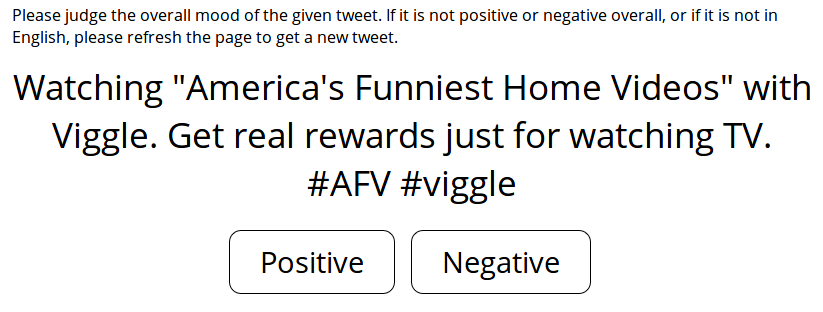
\includegraphics[width=470px]{figs/web_cat.png}

\subsubsection{Implementation}

When the page is loaded, a call is made to Twitter’s ``public timeline'' API \\
(\texttt{https://api.twitter.com/1/statuses/public\_timeline.json}), which returns approximately 20 of the most recent tweets posted. Each tweet is returned as a JSON object, with the text of the tweet itself, various statistics about it (such as whether or not it has been favorited), and a user object representing the author of the tweet.

Although some of the other Twitter APIs allow the caller to specify that they only want English tweets, this functionality did not work with \texttt{public\_timeline}. In order to display only English tweets to our users, we look at the ``lang'' field attached to the user object. After the code gets the list of tweets, it iterates through them until it finds one with a user who specified ``en'' as their language. Unfortunately, because the language specification is not on the tweet itself, because users may have specified their language incorrectly when signing up, and because users who primarily write in English may occassionally tweet in other languages, the tweets we displayed were not always actually in English. In cases where this happened, we instructed the viewer to simply refresh the page.

Once the user clicks on either ``positive'' or ``negative'' a POST call containing the user’s name, the text of the tweet, and a boolean specifying whether or not the tweet was positive is sent to the \texttt{write.php} script. This script writes to either \texttt{positive.txt} or \texttt{negative.txt} based on the boolean. In the specified file, it records the user’s name and the text of the tweet separated by a comma. Later, we manually took these files and merged them into one CSV file for training and testing.

\subsubsection{Possible Improvements}

The most obvious improvement in data collection would be to ensure that the tweets shown to the users are actually in English. Since the data collection through the web application was mostly completed by us, we didn’t feel it was necessary to implement better language checking. However, if we wanted to enlist a wider array of people to help with data collection, this would be a welcome improvement. Another improvement would be to strip out the commas (because commas are the delimiter in CSV files) and newlines (because each tweet should only be on one line) in tweets before saving them to the files. There were relatively few tweets that had one or both of these, so we corrected the data manually.

\subsection { Lexer }

One of the main assumptions of this project is that the chosen lexical units, in this case, words, are independent predictors of the classification of the Tweet.  This assumption cannot be correct, for something as complicated as language, but this does imply that the choice of partitioning the lexical units does matter.  Even after we have decided to use single-word lexemes, this leaves us with a few choices:

\begin{enumerate}[1)]
\item Do we maintain capitalization?
\item How do we handle ``\#hash'' keywords?
\item How do we handle emoticons like ``:)'', ``:('', and ``:')'' - these are the closest thing to a direct encoding of sentiment - so preserving them for the analysis is important!
\item How do we handle ``\&gt;'', ``\&lt;'', and other HTML entities?  These particular examples are interesting, because they are conventionally used to indicate something good (``\&gt;'') or bad (``\&lt;'').
\item How is regular punctuation reported?
\end{enumerate}

Our solution to these considerations was to break the text on the whitespace / punctuation characters, and lowercase everything.  In order to reasonably handle HTML entities, ``\&'' would be included with any tokens it prefixes, while ``;'' is ignored.  The other punctuation is grouped with adjacent punctuation, and each group reported as a separate word.  This handles the extremely informative punctuation such as emoticons, while also handling regular punctuation.  For example, it can be imagined that ``!'' might oftentimes terminate positive tweets, while ``...'' is used to terminate negative tweets.

Using these rules, we came up with a fairly concise Python function that we used throughout the Naive Bayes classifier to tokenize strings:

\begin{verbatim}

# Normalize by removing invalid characters (anything with an ASCII code
# outside the range [32, 126]).
# return filter( lambda x: x and ord(x) >= 32 and ord(x) <= 126 and x != '&' \
# Split on spaces, and then split on all non-alphabetical characters,
# except '&'.
def parse_tokens(input):
    dirty_tokens = sum([x.split(r'([^\w\&]+)') for x in input.split()], [])
    tokens = []
    for t in dirty_tokens:
        tokens.append(''.join(filter(valid_char, t)))
    return tokens

\end{verbatim}

\subsection { Bayesian Categorizer }

\subsubsection { Introduction }

Our Bayesian categorizer is implemented as a supervised machine learning algorithm, which is comprised of two steps: \textbf{preparing} the data by partitioning into a training set and a test set, and then \textbf{training} our Naive Bayes classifier on the training set in order to form a predictive model based on the observed probabilities of individual words occurring in a label. We can then test our predictive model on unlabeled test examples using the test set.

\subsubsection { Data Preparation }

Preparing and partitioning the data is implemented as a collection of Python scripts that take the labeled data from the web and console categorizers and re-formats it for the Naive Bayes classifier. Specifically, this involves organizing all the tweets into directories of individual files on disk, where each file contains exactly one tweet, and each directory corresponds to one label (positive or negative). The data is then partitioned into a training and test set by taking a random sample of 80\% of the data, using that for the training set, and moving the remaining 20\% into the test set.

\subsubsection { Training }

Once the data is processed and ready to learn, the Naive Bayes classifier trains itself by taking each tweet from the training data, splitting it into words using our lexer discussed in the previous section, and then recording the frequency of each word appearing in the tweet. In addition to the frequency, we also record the label of the tweet that the word appears in, so we can calculate prior probabilities for each word for each label.

As the classifier is building its predictive model, these frequencies are cumulatively aggregated. The end result is a model that consists of a bag of all words (and their frequencies) appearing at least once in a tweet, along with the labels they appeared in. For clarity, here is a short snippet from our classifier code:

\begin{verbatim}
# calculate word frequencies in each of the training examples
for filename, label in examples:
    category = self.categories[label]
    text = self.get_text(filename)
    for token in parse_tokens(text):
        category.freqs[token] += 1
        self.vocab.add(token)
        category.num_words += 1
    category.num_docs += 1
\end{verbatim}

Once we have these frequencies, for each label, we calculate the prior probabilities of each word being in a document that has that label by calculating how many times a word appeared in that label, divided by how many times that word appeared in all of the tweets. This gives us $P(F_i | C)$ for each word $F_i$ and label $C$. Calculating the probabilities 

\begin{verbatim}
def calculate_probabilities(self, freq_transform=lambda x: x):
    num_total_docs = sum(C.num_docs for C in self.categories.itervalues())
    for category in self.categories.itervalues():
        prob = float(category.num_docs) / num_total_docs
        category.prob = math.log(prob, 2)
        category.prob_word = {}
        for word in self.vocab:
            prob_word = \
              float(freq_transform(category.freqs.get(word, 0)) + 1) / \
                (category.num_words + len(self.vocab))
            if prob_word > 0:
                category.prob_word[word] = math.log(prob_word, 2)
\end{verbatim}

Then, when classifying an unlabeled test example, we use our simplified version of Bayes' theorem, as discussed earlier, to calculate $P(C | F_i)$ for all possible labels. We then choose the label that has the highest probability:

\begin{verbatim}
def classify_str(self, text):
    tokens = parse_tokens(text)
    probs = {}
    for label, category in self.categories.iteritems():
        probs[label] = category.prob
        for token in tokens:
            if token not in self.vocab:
                continue
            probs[label] += category.prob_word[token]
    argmax = max(probs.iteritems(), key=lambda x: x[1])
    return argmax
\end{verbatim}

\subsubsection { Implementation Notes }

One may notice from our probability calculation code that our particular implementation does not deal with actual likelihoods; instead, we only deal with log likelihoods in our code. This is because computing $P(F_1, ..., F_n | C)$ involves multiplying lots of probabilities. Since this is essentially multiplying lots of very small numbers, we rapidly lose accuracy due to numerical underflow and the limitations of binary floating point representation. Thus, we take the log of each probability and maximize their sum instead.

\subsection{Web Frontend}

\subsubsection{Introduction}
We also built a web frontend to demo our classifier. The web frontend was intended to show how our classifier behaves on arbitrary  user input. The user simply types text into the input box, and then clicks the ``Classify!'' button. A message will pop up with the result of the classification (either ``positive'' or ``negative'').

The web frontend can be accessed at: \texttt{http://abstract.cs.washington.edu/~coralp/stat391/classify.php}. A screenshot is shown below:

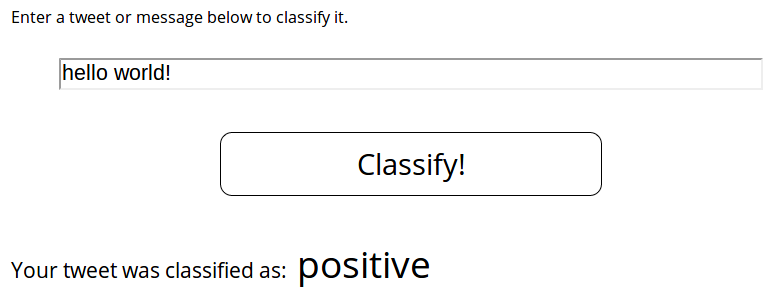
\includegraphics[width=470px]{figs/web_frontend.png}

\subsubsection{Implementation}
When the user clicks ``Classify!'', a script called \texttt{classify.js} gets the text that user entered and sends it to \texttt{get\_classification.php} as a GET request with the parameter ``text''. Before using the text value, the PHP script strips out apostrophes, because they cause syntax errors. After sanitizing the data, the script then calls the \texttt{naive\_bayes.py} Python script, giving it a previously saved model that is based on our training data, and passes the text of the tweet into the script. The Naive Bayes script finds the category that would best fit the given tweet, and returns the text string ``positive'' or ``negative''. The PHP script then takes this value and passes it back to the front-end code, which displays it in a text box for the user.

\subsubsection{Possible Improvements}
The most visible improvements would be to add more automatic suggestions to the demo. For instance, an option to pull the latest tweet and classify it would allow users to see the demo without thinking of something to write. The most recent tweet would also have the advantage of being data that is actually on Twitter; although users can theoretically write anything on Twitter, using data from the source instead of making it up on the spot would fit our previously collected data more clearly. Another possible improvement would be the ability to classify multiple tweets at a time. For instance, the ability to search for a hashtag and gauge the overal mood of tweets that use that hashtag would be an interesting exercise.

\section { Results }

\subsection{Overview}

In the end, we collected 627 data points, including 354 positive categorizations and 272 negative categorizations. This breakdown is illustrated in the following graph:

\begin{center}
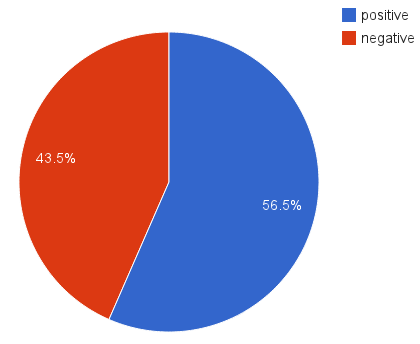
\includegraphics[width=300px]{figs/pos_neg_breakdown.png}
\end{center}

\begin{center}
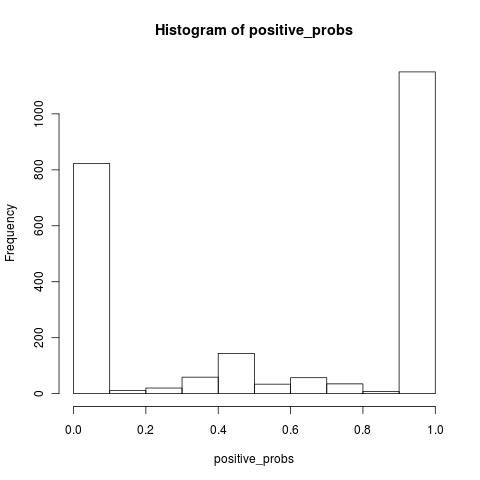
\includegraphics[width=300px]{figs/fig3.png}
\end{center}

The probability of a document being positive, given just the presence of one token, is the proportion of positive documents that contain that token.  The preceding graph is a histogram, showing the frequencies of these different probabilities.  The large extreme bars indicate that some words were only found in negative or positive posts.  Many of these are likely unique / rare tokens such as proper names.  However, this may also be an indication that more data would have been helpful.

Our classification accuracy is summarized by the following table:

\begin{tabular}{|l|l|}
\hline
\emph{Dataset} & \emph{Accuracy} \\ \hline
Training & 98.2\% \\ \hline
Test & 69.84\% \\ \hline
\end{tabular}

A more detailed breakdown is as follows:

\begin{tabular}{|l|l|l|l|l|}
\hline
\emph{Dataset} &
  \begin{tabular}[l]{@{}c@{}}\emph{Pos. examples}\\\emph{correctly classified}\\\emph{(\% of pos.)}\\\end{tabular} &
  \begin{tabular}[l]{@{}c@{}}\emph{Pos. examples}\\\emph{classified as neg.}\\\emph{(\% of pos.)}\\\end{tabular} &
  \begin{tabular}[l]{@{}c@{}}\emph{Neg. examples}\\\emph{correctly classified}\\\emph{(\% of neg.)}\\\end{tabular} &
  \begin{tabular}[l]{@{}c@{}}\emph{Neg. examples}\\\emph{classified as pos.}\\\emph{(\% of neg.)}\\\end{tabular}
  \\ \hline
Training & 280 (98.9\%) & 3 (1.1\%) & 211 (97.2\%) & 6 (2.8\%) \\ \hline
Test & 53 (74.6\%) & 18 (25.4\%) & 35 (63.6\%) & 20 (36.4\%) \\ \hline
\end{tabular}

\subsection{Discussion}

Our results weren't as good as we might have liked. Clearly, an accuracy of 69.84\% leaves something to be desired, and in any circumstance where tweets \emph{must} be classified with great accuracy, our classifier would be unsuitable. However, given the naïveté of our model we might have expected even worse. And given our experiences playing around with the web frontend, the classifier seems to perform reasonably well on any example we manually throw at it. Therefore, we might say that our classifier is ``good enough'' to perform broad categorization on tweets. In any case, our categories are highly subjective. So its hard to gage in the first place whether our labels were even correct.

It looks like, at least in the test set, more negative examples were misclassified than positive examples (on a percentage basis). This could be explained by the fact that, in general, we tended to manually classify examples as positive when we were unsure of their category. This would result in a bias within the classifier towards classifying examples as positive.

Tweets use ``hash-tag'' prefixes of words or compounded words in order to indicate some key-word relevant to the contents of your tweet.  In other words, this is a way to even further reduce the amount of content potentially included in your posts, while connecting your post to others'.

\section { Future Work }

Some ideas for enhancements:

\begin{enumerate}[1)]
\item Use bi-grams / tri-grams.  Instead of just making a distinct choice here, to use, say, bi-grams instead of uni-grams as the unit of association, it would be interesting to try to mix the categories.  When a particularly 

\item Use more sophisticated models to infer distributions that observe a co-dependency on terms.  In other words, find cases in which the presence of two words in the same tweet is significant, whereas each in isolation is not.

\item Use more sophisticated ways of extracting structure from the individual tweets.  Instead of parsing into tokens that are considered independently, parse into a tree that gives the actual relational structure of the text.  This could then be used to run some sort of trained semantic interpretation of the content.  One way in which this could dramatically affect results is by noticing negations like ``not'', which can entirely invert the sentiment of a Tweet.

\item Use context derivable from the edges derivable from the hash-tag / conversational graph.  This would further inform the previous enhancement idea.
\end{enumerate}

In essence, these further enhancements are each a more sophisticated usage / implementation of NLP (natural language processing) techniques, that would generically enhance many related categorization tasks.

\subsection { Max-Uncertainty Queue }

One issue with this project is that, similarly to many studies, there is cost associated with taking additional samples.

In the case Mechanical turk, the cost was $ \$1.16 / 40 \text{ tweets} ~ \$0.029 \text{ tweets}^{-1}$. 

%TODO: consider measuring this better.

In the case of using the manual categorizer, we found that we could categorize tweets at about a rate of about $ 15 \text{ tweets} / \text{min} $.  This means that with a solid hour of work, we could categorize 900 tweets.  In order to compute what this means for our price per tweet, we first need an estimate of the value of our time.  If our time is worth the pay of a typical entry-level full-time software engineer, $ \$40 / \text{hr} $, then each tweet costs $ \$40 \text{min}^{-1} / ( 900 \text{ tweets} * \text{min}^-1 \approx \$0.045 * \text{tweets}^-1 $.  However, we are all in school!  Perhaps it would be more appropriate to use the amount made as a TA: $ \$10.50 * \text{min}^{-1} / ( 900 * \text{tweets} * \text{min}^{-1} ) \approx \$0.015 $.  This is around half as much as the cost of Mechanical Turk, which incentive us to do more manual than ``mechanized'' sampling.

Either way, it would be cool to make the most of the resource expenditure involved in categorization.  An interesting way of approaching this problem would be to write it down as an optimization problem that relates the overall value of taking a sample to the potential for information gain and cost of collection:

\begin{align*}
V = P_u * U(F_1,\dots,F_n) - P(F_1,\dots,F_n)
\end{align*}

where $ U(F_1,\dots,F_n) $ is some approximation of the amount of uncertainty involved in classifying a document with the features $ F_1,\dots,F_n $, and $ P(F_1,\dots,F_n) $ is the cost of human classification.  $ P_u $ is a coefficient which determines the dollar value of a reduction in uncertainty.  A definition for $ U $ might looks something like:

\begin{align*}
U(F_1,\dots,F_n) = \frac {1} {\frac{N_1}{\vert 0.5 - P(F_1 \vert C_1) \vert} + \dots + \frac{N_n}{\vert 0.5 - P(F_n \vert C_1) \vert}}
\end{align*}

\subsection { Sparsity assumptions }

A more recent development in sensor post-processing / learning models is an idea that's referred to as \emph{compressive sensing}, which attempts to recover more accurate models by assuming that the process being studied is \emph{sparse}.  Many continuous optimization problems can be posed in terms of something similar to the $ L_2 $ norm (e.g. least squares)  This norm creates surfaces that resemble a cone.  As such, if you fix any of the parameters, you get conic,   The key observation of \emph{compressive sensing} is that optimizing things that much more resemble the structure of the linear norm, $ L_1 $, creates more extreme slopes along the axii, encouraging settling there.  This encourages values to be set to zero, hence the word \emph{sparsity}.  Technically, sparsity would involve minimizing the $ L_0 $ norm, which corresponds to the number of non-zero elements of the vector.  However, this becomes a very difficult, combinatorially complex, discrete optimization problem (on a space with cardinality $ | \{T, F\}^n | =  2^n $).  Researchers have come up with efficient ways of minimizing the $ L_1 $ norm and have shown that $ L_1 $ is a good approximation for minimizing $ L_0 $.

Sparsity is interesting for a number of reasons.  One is that it is a good optimization.  If we adopt a sparse representation for the learned model, then evaluating the model consists of iterating its non-zero elements.  Another benefit is that for some domains, sparsity is a reasonable assumption, as there is some underlying cause for the input, with added noise.

This is the reason that these considerations are relevant - it gives a philosophical motivation for systematically ignoring some of the features in our model.  We can imagine running an optimization that determines the probability used to represent a particular $ P(F_i \vert C) $.  This would deviate from the probability indicated by the actual frequency, as a cost function related to the overall distance from $ 0.5 $ would be applied.  In other words, you need to ``buy'' discriminatory power, under the assumption that the weak features are noisy disinformation.

As a first approximation, to test whether this idea might have some value to it for this application, we removed the features that weren't highly dichotomized.  This was done by removing the features that satisfy $ \vert \frac{P(F_i \vert C_1)}{P(F_i \vert C_1) + P(F_i \vert C_2)} - 0.5 \vert \leq \delta $, where $ \delta $ is the distance from $ 0.5 $ that should be cropped.

Unfortunately, strangely, no value of $ \delta $ yielded an increase in the performance of the classifier on the test data.  It's possible that pursuing a more theoretically grounded approach to this, that also takes into account the quantity of samples involving the feature, would yield better results.

% \subsubsection{ Graphical Models }

% The study of graphical models involves the crossover between graph theory and probability theory, and gives a uniform perspective of many techniques for creating models and categorizers.  These models express dependencies between states of various nature relating to a system - in the case of ``Partially Observable Markov Decision Processes'', this includes observations and states.  The dependencies among the states indicate the temporal interdependencies of the states, while also being informed by the observations.  The current state of the belief distribution is used as an input, along with these observations, to evaluate the joint probabilities at each state, of now inhabiting that state.  Thankfully, our model does not need to worry about anything quite like these temporal dependencies (but if we worried about context, something like this would be needed!).

% Anyway, since our system is merely Naive Bayes, it can be expressed quite trivially as a graphical model:

% \input { figs/fig1.tex }

\end{document}